Para el problema de devolver un conjunto de bundles diversos y complementarios sujeto a un presupuesto se implementó el algoritmo Produce-and-Choose (PAC) sugerido en el artículo \cite{compositeRetrival} consiste en generar un conjunto de bundles y luego elegir el posible mejor subconjunto para que sea la solución. Adicionalmente se desarrolló un algoritmo goloso en el que la solución se construye seleccionando el ítem que maximiza la función objetivo en cada paso.\\
En pos de mejorar las soluciones obtenidas se implantaron dos metaheurísticas de la familia de la búsqueda tabú. La primera tiene como objetivo encontrar mejores bundles en la etapa de producción del algoritmo PAC. Mientras que la segunda explora las soluciones vecinas de un resultado dado.\\
\section{Modelo}
Dado el conjunto de objetos $I$ y una función de similitud $ s: I \times I \rightarrow [0;1]$, cada objeto es unívocamente identificado y contiene un conjunto de atributos. La entrada puede pensarse como un grafo completo con peso en las aristas $G=(I,E,s)$ donde el peso del vértice $(u,v)$ es $s(u,v)$. Se define también la \textit{función de distancia} $d(u,v) = 1 - s(u,v)$ que también toma valores en el intervalo $[0;1]$.

\section{Problema}
El problema consiste en devolver un conjunto de bundles $S = \left\{s_1, \ldots, s_k\right\}$ donde el bundle $S_i \in 2^{I}$ es un conjunto de objetos que satisface las reglas de \textit{complementaridad} que no permite que existen dos objetos con igual atributo en el mismo bundle y de \textit{presupuesto} para que la suma de los costos de los objetos no exceda el presupuesto dado.\\
\textbf{Definición} Dado el conjunto de objetos $I=\left\{i_1,\ldots, i_n\right\}$ el bundle $S \in 2^{I}$ es válido si y sólo si satisface las reglas:
\begin{itemize}
	\item \textbf{Complementaridad:} dada la propiedad $\alpha$ de los objetos, $\forall u,v \in S_i, u.\alpha \neq v.\alpha$
	\item \textbf{Presupuesto:} dada la función de costo $f$ y el presupuesto $\beta$, entonces $\forall S_i \in S, f(S_i) \leq \beta$
\end{itemize}

La definición formal de \textit{Composite Retrieval} es:\\
Dado el conjunto de objetos $I = \left\{i_1, \ldots, i_n \right\}$, la función de similitud $s(u,v)$, el atributo complementario $\alpha$, la función de costo $f$, el presupuesto $\beta$ y el entero $k$ se desea hallar el conjunto válido de bundles $S = \left\{s_1, \ldots, s_k\right\}$ que maximiza la función:
\begin{equation} \label{des:eq-fnObj}
  \sum_{1 \leq i \leq k}{\sum_{u,v \in S_i}{\gamma s(u,v)}} + \sum_{1 \leq i \leq j \leq k}{(1-\gamma) (1-\max_{u \in S_i, v \in S_j}{s(u,v)})}
\end{equation}
Esta es una tipia función objetivo de un problema de clustering, donde la calidad del clustering es una combinación entre la calidad de cada cluster (intra-cluster) y de la separación entre clusters (inter-cluster). A través del parámetro $\gamma$ el usuario puede definir el balance entre intra e inter de una solución. Si El usuario prioriza una solución de bundles cohesivos sobre la diversidad el  valor de $\gamma$ será cerca de uno y si lo que prioriza es la diversidad el valor estará cerca del cero.\\
En \cite{compositeRetrival} se demuestra que la complejidad de devolver $k$ bundles de items complementarios con un presupuesto es NP-Completo, por el momento no se puede encontrar una solución exacta en tiempo polinomial, por lo cual este trabajo se enfoca a encontrar soluciones suficientemente buenas para el problema. Para poder encontrar la mejor solución se implementaron dos algoritmos para poder comparar los resultados: Produce-and-Choose y algoritmo goloso.

\section{Produce-and-Choose}
El algoritmo para aproximar a la solución \texttt{Produce-and-Choose} generá una cierta cantidad de bundles y luego selecciona los bundles de la solución.\\

Los parámetros del algoritmo son los del problema: $I$ el conjunto de ítems, $\alpha$ el atributo complementario, $f: 2^{I} \rightarrow \rm I \!R$ la función de presupuesto, $\beta$ el limite del presupuesto, $\mu$ el umbral del valor del intra a superar por cada bundle y $c$ la cantidad de bundles a generar. El algoritmo devuelve un conjunto de bundles válidos.\\
\begin{algorithm}[H]
\begin{algorithmic}[1]
\REQUIRE {$I,\alpha,f,\beta,k,\gamma$}
\ENSURE Conjunto válido de $k$ bundles
\STATE $Cand \leftarrow ProduceBundle(I,\alpha,f,\beta)$
\STATE $G \leftarrow BuildBundleGraph(Cand)$
\RETURN $ChooseBundles(k,\gamma,G)$
\end{algorithmic}
\caption{Produce-and-Choose}\label{alg:PAC}
\end{algorithm}

\subsection{Generación de bundles}
La generación de bundles se puede realizar a través de un proceso de agrupación de un conjunto de objetos que son parecidos. Este proceso es conocido como clustering, que consiste en agrupar objetos basándose en la información que estos describen o en sus relaciones. El objetivo es que los objetos del cluster sean similares entre sí y diferentes de los objetos de los otros grupos. Cuanto mayor es la similitud en el cluster (intra) y mayor la diferencia entre los cluster (inter) es mejor la clusterización.\\
No existe una definición formal de que es un cluster correctamente constituido porque es muy complejo realizar esta definición. Por ejemplo, para los veinte puntos de la figura \ref{res:img-howToCluster} existen tres (o más) formas de clusterizar que son válidas. Si se permite que los cluster estén acoplados, entonces la estructura de los cluster más razonable es en la que hay dos clusteres. Pero la división de los dos clusteres en tres subclusters es más intuitiva para el ojo humano. Tampoco es irracional decir que los puntos pertenecen a cuatro clusteres. Entonces la mejor definición depende del tipo de dato y del resultado esperado.


\begin{figure}[H]
  \centering
   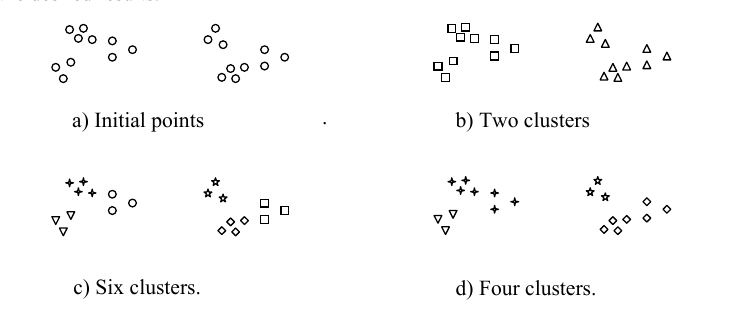
\includegraphics[width=0.8\textwidth]{img/howToCluster.png}
   \caption{}
   \label{res:img-howToCluster}
\end{figure}

En la clusterización para Composite Retrieval, la definición es que cada cluster maximice el costo indicado y que no cambiará en la ejecución de la búsqueda, pues lo esperado es obtener distintos clusters que hayan utilizado el máximo del presupuesto. El criterio utilizado para realizar la agrupación es a través de la similitud entre los objetos del universo, ésta será representada por una función logrando que los clusters obtenidos sean lo mas parecidos posibles entre ellos, logrando de esta manera bundles cohesivos.\\
Existen varios algoritmos de clustering, los cuales se pueden categorizar entre los particionales y los jerárquicos. Los métodos particionales reubican iterativamente los objetos moviéndolos de un cluster a otro. Generalmente, estos métodos, requieren que la cantidad de cluster a generar sea preestablecido. Los métodos jerárquicos construyen los clusteres mediante la partición recursiva de los grupos de objetos y no requieren preestablecer la cantidad de cluster.\\
En este trabajo se implementó un algoritmo de cada categoría. Del método jerárquico se desarrolló el algoritmo \textit{constrained hierarchical agglomerative clustering}, mientras que para el método de partición el algoritmo \textit{Bundles One-By-One}.\\

\subsubsection{Bundles One-By-One}
El método \texttt{BOBO-k}, que está inspirado en k-means, consiste en generar $k$ cluster del conjunto de $n$ ítems. El algoritmo comienza con todos los items del conjunto $I$ como posibles pivots $P$. Se selecciona un pivote de $P$ y con los elementos de $I$ se genera un bundle válido alrededor de este, en caso que el bundle generado sea suficientemente bueno se agrega al conjunto de bundles candidatos y los ítems del bundle se eliminan de $I$. La generación de bundles continúa hasta que se cumpla el criterio de parada que es la generación de $k$ bundles. Con \texttt{BOBO-k} pueden quedar items excluidos de los bundles generados, por lo tanto se desarrolló una variante del método que es el \texttt{BOBO-Ex} (Ex de \textit{exhaustive}) en el cual todos los items pertenecen a un bundle. Para esta producción se modificó el criterio de parada hasta que el conjunto de pivotes $P$ sea vacío.\\

\begin{algorithm}[H]
\begin{algorithmic}[1]
\REQUIRE {$I,\alpha,f,\beta,\mu,$ cantidad de bundles $c$}
\ENSURE Conjunto válido de bundles
\STATE $P \leftarrow I$
\STATE $C \leftarrow \emptyset$
\WHILE {$ \left|C\right| < c\ and\ P \neq \emptyset$}
	\STATE $p \leftarrow selPivote(P)$
	\STATE $b \leftarrow generarBundle(p,I,\alpha,f,\beta)$
	\IF {$score(b) \geq \mu$}
		\STATE $C \leftarrow C \cup \left\{b\right\}$
		\STATE $I \leftarrow I \setminus b$
		\STATE $P \leftarrow P \setminus b$
	\ELSE
		\STATE $P \leftarrow P \setminus \left\{p\right\}$
	\ENDIF
\ENDWHILE
\RETURN $C$
\end{algorithmic}
\caption{BOBO-k}\label{alg:bobo}
\end{algorithm}

La función \texttt{selPivote} selecciona el pivote del conjunto de pivotes, en este trabajo se siguió con la recomendación de \cite{newSimilarity} que la selección sea aleatoria. La función \texttt{generarBundle} genera un bundle a partir del pivote. Se trata de una función que implementa un algoritmo goloso dado que que en cada iteración se agrega al bundle que se genera el ítem del conjunto $I$ que maximiza la función intra $f$ y que cumple con las restricciones de la complementaridad y el presupuesto. La función \texttt{score} calcula el valor intra del bundle. Se dice que un bundle es suficientemente bueno si el valor intra supera el umbral establecido por $\mu$.\\

\subsubsection{Constrained hierarchical agglomerative clustering}
La clusterización jerárquicos se clasifica entre los algoritmos \textit{aglomerativo} y \textit{divisivo}. En el aglomerativo inicialmente cada objeto pertenece a un cluster unitario y luego sucesivamente se unen un par de clusters hasta que todos los clusters se hayan unido en un único cluster que contenga a todos los objetos, esete algoritmo es conocido como \textit{hierarchical agglomerative clustering} (HAC). El divisorio comienza con un único cluster al que todos los objetos pertenecen y recursivamente se realiza una división del cluster hasta obtener clusters con un solo objeto.\\
Comúnmente HAC es visualizado como un dendrograma, como se ve en la figura ~\ref{des:Dendrogram}, cada unión se representa por una línea horizontal y la coordenada Y es la similitud en la que los dos clusters han sido unidos. Por ejemplo la unión del cluster que contiene a \textit{Indiana tobacco lawsuit} con el cluster de \textit{Suits against tobacco firms}, es con la similitud aproximada de 0,7. Luego el cluster resultante se une con el cluster de \textit{Lawsuit against tobacco companies} con la similitud 0,47. Sucesivamente se realizan la unión de estos cluster hasta que quede uno solo.\\
Ascendiendo desde la capa inferior hasta obtener un único cluster el dendrograma permite reconstruir la historia de las uniones de los clusters. Un supuesto fundamental en el algoritmo HAC es que es monótono, lo que significa que si la unión sucesiva de cluster es con las similitudes es $s_1,s_2,\ldots,s_n$ entonces se tiene que $s_1 \geq s_2 \geq \ldots \geq s_n$.\\

\begin{figure}[H]
  \centering
    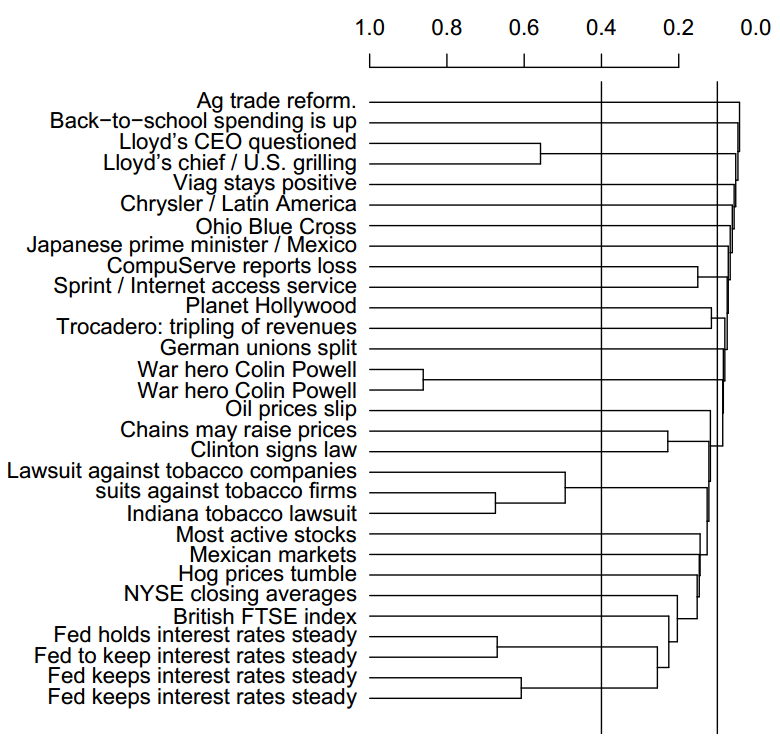
\includegraphics[width=1\textwidth]{img/Dendrogram.png}
  \caption{dendrograma}
  \label{des:Dendrogram}
\end{figure}

\textit{Constrained hierarchical agglomerative clustering} (C-HAC) es una modificación que se realiza sobre HAC para que nunca se realice la unión de los clusters $S_1$ y $S_2$ si el cluster resultante $S_1 \cup S_2$ es inválido, o sea sí el cluster resultante no cumple con las restricciones de similitud o el costo del bundle supera el presupuesto. El algoritmo C-HAC que se presenta a continuación, en este trabajo se denomina \texttt{Simple C-HAC}, es el que se propone en \cite{compositeRetrival} tiene la misma entrada y salida que el algorito \texttt{BOBO-k} .\\

\begin{algorithm}[H]
\begin{algorithmic}[1]
\REQUIRE {$I,\alpha,f,\beta,$ cantidad de bundles $c$}
\ENSURE Conjunto válido de bundles
\STATE $Cand \leftarrow \bigcup_{i \in I}\left\{i\right\}$
\WHILE {$ \left|Cand\right| > c$}
	\STATE $bestcore \leftarrow -\infty$
	\STATE $bestcandidate \leftarrow \emptyset$
	\FOR{each $S_i\in Cand$}
		\FOR{each $S_j\in Cand; S_i \neq S_j$}
			\IF {$validMerge(S_i,S_j,\alpha,f,\beta)$} \label{validMerge}
				\IF {$score(S_i \cup S_j) \geq bestcore$} \label{score}
					\STATE $bestcore \leftarrow score(S_i,S_j)$
					\STATE $bestcandidate \leftarrow \left\{S_i,S_j\right\}$
				\ENDIF
			\ENDIF
		\ENDFOR
	\ENDFOR
	\IF {$bestcandidate = \emptyset$}
		\BREAK
	\ENDIF
	\STATE {$Cand \leftarrow Cand \setminus \left\{S\right\}$ $\forall S \in bestcandidate$}
	\STATE $Cand \leftarrow Cand \cup bestcandidate $
\ENDWHILE
\RETURN $Cand$
\end{algorithmic}
\caption{Simple C-HAC}\label{alg:SimpleC-HAC}
\end{algorithm}

El algoritmo ejecuta $N - c$ pasos donde se unen los dos clusters más similares que forman un cluster válido. En cada paso se realiza una comparación entre todos los clusters. Por lo tanto el orden de complejidad de \texttt{Simple C-HAC} es $\mathcal{O}(N^{3})$.\\

La función \textit{score} devuelve la similitud entre dos clusters. Para realizar esta medición se plantearon dos alternativas: \textit{single-link} y \textit{complete-link}.\\

En \textit{single-link}, la similitud entre dos clusters es la similitud de los miembros más similares. Este criterio de unión es local, ya que solo se presta atención al área dónde los dos clusters están mas cerca.\\

En \textit{complete-link}, el par de cluster que se selecciona para unir es el que maximiza la función objetivo. Por lo tanto este criterio no es local, la estructura del clustering influye en la decisión de cuales son los cluster a unir.\\

La figura ~\ref{des:LinkageCriteria} representa el comportamiento de los criterios \textit{single-link} y \textit{complete-link} en el proceso de clusterización de ocho objetos. Cada elipse corresponde a un paso sucesivo de la clusterización. En los primeros cuatro pasos los cluster generados son iguales. En \textit{single-link} se unen el par de clusters de arriba (después el par de abajo) porque la similitud entre los objetos $d_2$ y $d_3$ es mayor a la similitud entre $d_2$ y $d_6$. Mientras que \textit{Complete-link} une el par de clusters de la izquierda (después el par de la derecha) porque la similitud entre 
 $d_1$ y $d_4$ es menor a la similitud entre $d_1$ y $d_6$.\\

\begin{figure}[H]
  \centering
    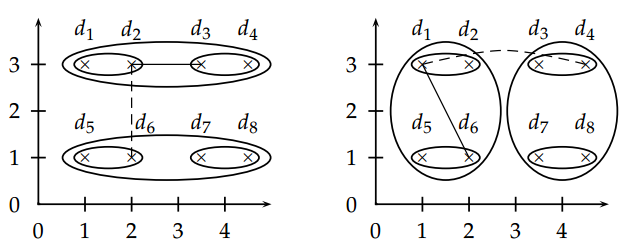
\includegraphics[width=1\textwidth]{img/LinkageCriteria.png}
  \caption{single-link (izquierda) y complete-link (derecha)}
  \label{des:LinkageCriteria}
\end{figure}


Por el orden de complejidad del algoritmo \texttt{Simple C-HAC}  en escenarios donde la clusterización se tenga que hacer entre miles de objetos el tiempo de ejecución será tan elevado que el algoritmo es improductivo. Para contemplar estos escenarios se implemento el algoritmo \texttt{Efficient C-HAC} que la complejidad es $\mathcal{O}(N^{2}\lg n)$. La similitud entre los clusters se guarda en colas de prioridad en orden decreciente, entonces la cola $P\left[k\right].max()$ devuelve el cluster de mayor similitud con el k-ésimo cluster. Luego de combinar los clusters $\omega_{k_{1}}$ y $\omega_{k_{2}}$, $\omega_{k_{1}}$ se utiliza como la representación. Para $\omega_{k_{1}}$ se calcula la similitud con el resto de los clusters y se actualiza en las colas de similitud. Para identificar entre dos cluster que la unión es invalida por alguna de las restricciones, en las colas de similitud el valor de la similitud es $-1$.\\

\begin{algorithm}[H]
\begin{algorithmic}[1]
\REQUIRE {$I,\alpha,f,\beta$}
\ENSURE Conjunto válido de bundles
\FOR{each $S_i\in I$}
	\FOR{each $S_j\in I$}
		\IF {$validMerge(S_i,S_j,\alpha,f,\beta)$} 
			\STATE $C[i][j].sim \leftarrow score(S_i \cup S_j)$
		\ELSE
			\STATE $C[i][j].sim \leftarrow -1$
		\ENDIF
		\STATE $C[i][j].index \leftarrow j$
	\ENDFOR
	\STATE $I[i] \leftarrow 1$
	\STATE {$P[i] \leftarrow $ priority queue for $C[i]$ sorted on sim}
	\STATE {P[i].Delete(C[i][i]) (se elimina así mismo de la pila)}
\ENDFOR
\STATE $A \leftarrow []$
\FOR {$k \leftarrow 1$ to $I.length$}
	\STATE $k_1 \leftarrow \max_{k:I[k]=1}{P[k].max().sim}$
	\IF {$validMerge(S_i,S_j,\alpha,f,\beta)$}
		\BREAK
	\ENDIF
	\STATE $k_2 \leftarrow P[k_1].max().index$
	\STATE $A.Append(\left\langle k_1,k_2 \right\rangle)$
	\STATE $I[k_2] \leftarrow 0$
	\STATE $P[k_1] \leftarrow []$
	\FOR {$i$ with $I[i]-1 \vee i \neq k_1$}
		\STATE $P[i].Delete(C[i][K_1])$
		\STATE $P[i].Delete(C[i][k_2])$
		\IF {$validMerge(S_i,S_j,\alpha,f,\beta)$}
			\STATE $C[i][k_1].sim \leftarrow score(i,k_1,k_2)$
			\STATE $C[k_1][i].sim \leftarrow score(i,k_1,k_2)$
		\ELSE
			\STATE $C[i][k_1].sim \leftarrow -1$
			\STATE $C[k_1][i].sim \leftarrow -1$
		\ENDIF
		\STATE $C[i][k_1].index \leftarrow i$
		\STATE $C[k_1][i].index \leftarrow i$		
		\STATE $P[i].Insert(C[i][k_1])$
		\STATE $P[K_1].Insert(C[k_1][i])$		
	\ENDFOR
\ENDFOR

\RETURN $A$
\end{algorithmic}
\caption{Efficient C-HAC}\label{alg:Efficient C-HAC}
\end{algorithm}

\subsection{Selección de bundles}
Al finalizar la producción de bundles comienza la etapa de selección de bundles en la cual se deben seleccionar los $k$ bundles para la solución. El problema de seleccionar los bundles que maximizan la función objetivo se traduce en encontrar en el grafo completo G con peso en los nodos y vértices (el peso de los nodos representa la calidad de los bundles y el peso de las aristas es la distancia entre los nodos) el k-subgrafo de mayor peso (considerando los nodos y vértices).\\
Formalmente el problema de encontrar el subgrafo de máximo peso de nodos y vértices con k nodos, consiste en dado el grafo $ G = (V,E) $, la funciones de peso $\psi : E \rightarrow \Re$ y $\omega : V \rightarrow \Re$, el entero $ k \leq |V| $ y el real $\gamma \in [0,1]$. La salida es el conjunto $V' \subseteq V$ tal que $|V'| = k$ que maximiza el peso de los nodos y vértices del subgrafo $G' = (V', E')$ ponderado por el parámetro $\gamma$.

\begin{equation}
\gamma \sum_{v \in V'}{\omega(v)} + (1 - \gamma) \sum_{(u,v) \in E'}{\psi(u,v)}
\end{equation}

El problema de encontrar el máximo k-subgrafo con pesos en los nodos y vértices, se puede reducir al problema ya conocido de hallar el k-subgrafo más denso\cite{SubgraphProblem}. Transformando en la instancia del problema original la función del peso de los vértices por:
 
\begin{equation}
\omega(u,v) = \dfrac{\gamma}{2( k - 1)} (\omega(u) + \omega(v)) + (1 - \gamma)\psi(u,v) 
\end{equation}

A esta nueva instancia del problema se le aplica la heurística golosa, del artículo \cite{compositeRetrival}, en la que en cada iteración se remueve el nodo con menos peso en las aristas.\\

\begin{algorithm}[H]
\begin{algorithmic}[1]
\REQUIRE $k,\alpha,$ el grafo con peso en los vértices y aristas  $G=(V,E)$ donde $\forall S \in V / \omega(S) = \sum_{u,v \in S}{s(u,v)}$ y $\forall (S_i,S_j) \in E / \psi(S_i,S_j) = 1 - \max_{u \in S_i, v \in s_j}{s(u,v)}$
\ENSURE Conjunto de k bundles
\STATE $\omega(u,v) = \dfrac{\gamma}{2( k - 1)} (\omega(u) + \omega(v)) + (1 - \gamma)\psi(u,v)$
\STATE $S \leftarrow V$
\WHILE {$ \left|S\right| > k$}
\STATE $u \leftarrow \min_{u \in S}{\sum_{v \in S}{\omega(u,v)}}$
\STATE $S \leftarrow S \setminus  \left\{u\right\} $
\ENDWHILE
\RETURN $C$
\end{algorithmic}
\caption{Selección de bundles}\label{alg:chooseBundles}
\end{algorithm}

En este trabajo se propone otra heurística para la selección que consiste en ir seleccionando iterativamente los bundles de la solución. En cada iteración se elije al bundle que maximiza la función objetivo, a diferencia del algoritmo ~\ref{alg:chooseBundles}, multiplicada por un coeficiente para ponderar la parte inter de la función. Esta ponderación se realiza porque el peso del nodo (parte intra de la función) es mayor al peso de la arista (parte inter). Con este equilibrio se asegura que en las primeras iteraciones el valor del intra no haga despreciable al inter en el momento de realizar la selección.\\
Sea $B$ el conjunto de bundles producidos y $S \subseteq B$ el conjunto de bundles seleccionados en la iteración $i$ se agrega a la solución el bundle que cumple con:

\begin{equation}
\max_{b \in (B/S)}{\dfrac{k}{|S|}} \gamma \sum_{v \in \left\{b\right\} \cup S}{\omega(v)} + \dfrac{k * (k-1)}{|S| * (|S|-1)} (1-\gamma) \sum_{v,w \in \left\{b\right\} \cup S}{\psi(v,w)}
\end{equation}

\begin{algorithm}[H]
\begin{algorithmic}[1]
\REQUIRE $B,k$
\ENSURE Conjunto de k bundles
\STATE $S \leftarrow V$
\WHILE {$ \left|S\right| < k$}
\STATE $c \leftarrow \max_{b \in (B/S)}{\dfrac{k}{|S|}} \gamma \sum_{v \in \left\{b\right\} \cup S}{\omega(v)} + \dfrac{k * (k-1)}{|S| * (|S|-1)} (1-\gamma) \sum_{v,w \in \left\{b\right\} \cup S}{\psi(v,w)}$
\STATE $S \leftarrow S \cup \left\{c\right\}$
\STATE $B \leftarrow B \setminus \left\{c\right\}$
\ENDWHILE
\RETURN $S$
\end{algorithmic}
\caption{Selección de bundles proporcional}\label{alg:algSelProp}
\end{algorithm}

\section{Algoritmo goloso}
Por la forma de generar la solución que tiene la heurística \texttt{Produce-and-choose} de construir una cantidad suficiente bundles y luego seleccionar un conjunto se puede suponer que las soluciones se enfocan más en la parte intra que inter. Esto motivo a realizar una otra heurística.\\
La heuristica que se propone es un algoritmo goloso, se generan únicamente los bundles que pertenecen a la solución, que agrega iterativamente el item al bundle que maximiza la función objetivo, aceptando que la función objetivo disminuya de un paso a otro. El algoritmo comienza con los bundles de la solución vacíos y en cada paso se selecciona el item que agregándolo a uno de los bundles maximiza la función objetivo y sin violar las restricciones del problema. El algoritmo finaliza cuando por alguna restricción no es posible agregar más objetos a la solución.

\begin{algorithm}[H]
\begin{algorithmic}[1]
\REQUIRE {$I,\alpha,f,\beta,$ cantidad de bundles $c$}
\ENSURE Conjunto válido de bundles
\STATE $Cand \leftarrow \bigcup_{1 \ldots c}\emptyset$
\STATE $isComplete \leftarrow False$
\WHILE {$isComplete = False$}
  \STATE $bestScore \leftarrow -\infty$
  \STATE $bestElement \leftarrow \varnothing$
  \STATE $bestBundle \leftarrow \varnothing$
  \FOR {each $elem \in I$}
    \FOR {each $bundle \in cand$}
      \IF {$isValidBundle(bundle \cup \{elem\})$}
        \STATE $score \leftarrow FO((Cand \setminus \left\{bundle\right\}) \cup \left\{bundle \cup \left\{elem\right\}\right\})$
        \IF {$score > bestScore$}
          \STATE $bestScore \leftarrow score$
          \STATE $bestBundle \leftarrow bundle$
          \STATE $bestElement \leftarrow elem$
        \ENDIF
      \ENDIF
    \ENDFOR
  \ENDFOR
	\IF {$bestElement \neq \varnothing$}
		\STATE $Cand \leftarrow (Cand \setminus \left\{bestBundle\right\}) \cup \left\{bundle \cup \left\{bestElement\right\}\right\}$
		\STATE $I \leftarrow I \setminus \left\{bestElement\right\}$
	\ELSE
		\STATE $isComplete \leftarrow True$
	\ENDIF
\ENDWHILE
\RETURN $Cand$
\end{algorithmic}
\caption{Algoritmo heurística golosa}\label{alg:algHeuGol}
\end{algorithm}

\section{Búsquedas Tabú}
Las búsquedas locales consisten en moverse de solución en solución, aplicando cambios a la solución candidata hasta encontrar una mejor solución o satisfacer un criterio de parada. Los algoritmos consisten en comenzar con una solución e iterativamente moverse a una solución vecina, esto es posible solo si se pude definir una relación de vecindad en el espacio de búsqueda. Como una solución puede tener muchas soluciones vecinas se elige siempre la que maximice o minimice (según el problema elegido) el criterio seleccionado, esto produce que el algoritmo pueda estancarse en un mínimo (ó máximo) local y nunca pueda salir de él.\\
\textbf{Tabú search} es una metaheurística, de la familia de las búsquedas locales, que relaja la primer regla de las búsquedas locales tradicionales y permite moverse a una solución vecina que no cumple con el criterio de búsqueda. De esta manera se permite al algoritmo escapar de máximos o mínimos locales y encontrar una mejor solución (en caso que existiese). Otras de las modificaciones que se agregan es que una vez que una solución determinada es visitada, se la marca como tabú para que no vuelva a ser visitada por una determinada cantidad de iteraciones para también de esta manera evitar caer en ciclos y mínimos o máximos locales.\\
Una de las ventajas que tienen este tipo de metaheurísticas es que no son muy costosas en tiempo de ejecución siempre que la cantidad máxima de iteraciones no sea excesiva, con lo cual se puede ejecutar sin problemas y sin importar el algoritmo de generación y selección provenga la solución orginal con el fin de intentar mejorarla.\\
Se implementaron las búsquedas tabú Inter-Bundle e Intra-Bundle. La primera busca encontrar una mejor solución entre la solución actual y los bundles ya generados; la otra consiste en mejorar los bundles con los items que quedaron fuera de la solución.

\subsection{Inter-Bundle}
La búsqueda se concibió especialmente para la fase de selección del algoritmo \texttt{Produce and Choose}. En esta fase se eligen los bundles que pertenecen a la solución. De la solución obtenida se realiza la búsqueda tabú con los bundles generados en la fase del produce con el objetivo de recorrer las soluciones con bundles menos cohesivos entre si.\\
Los movimientos de la solución $S$ a la solución $S'$ consiste de los siguientes  pasos:
\begin{enumerate}
	\item Obtener el Bundle de la solución a reemplazar.
	\item Determinar el bundle centroide de la solución.
	\item Agregar a la solución el bundle más alejado al centroide.
\end{enumerate}

Sea $S$ el conjunto de bundles de la solucion y B el conjunto de todos los bundles producidos. El bundle (1) es el más acoplado al de la solución $b_r = \min_{b_1 \in S}{\sum_{b_2 \in S}{\psi(b_1,b_2)}}$. El centroide de (2) es el bundle que tiene mayor similitud entre los bundles de la solución, sin tener en cuenta al bundle a reemplazar, entonces el centroide es:
$$b_c = \min_{b_1 \in S \setminus \left\{b_r\right\}}{\sum_{b_2 \in S \setminus \left\{b_r\right\}}{\psi(b_1,b_2)}}$$
El bundle de (3) se obtiene de $b_n = \min_{b_1 \in S \setminus \left\{b_r\right\}}{\psi(b_1,b_c)}$. Por lo tanto la nueva solución es $S' = (S \setminus \left\{b_r\right\}) \cup \left\{b_n\right\}$. Mientras que el bundle $b_r$ se marca para que no sea seleccionado para las próximas soluciones generadas.
\begin{algorithm}[H]
\begin{algorithmic}[1]
\REQUIRE $aSolution: Vector<SnowFlake>, $\\
         $remainingBundles: Vector<SnowFlake>, gamma: Double$
\ENSURE $newSolution:Vector<SnowFlake>$
\STATE $iteration:Integer \leftarrow 0$
\STATE $tabuBundles: Set<SnowFlake>$
\STATE $bestSolution: Vector<SnowFlake> \leftarrow aSolution$
\STATE $bestFunction:Double \leftarrow FO(bestSolution)$
\STATE $tempSolution: Vector<SnowFlake> \leftarrow bestSolution$
\WHILE {$iteration < MAX\_ITER$}
  \STATE $updateTabuCount(tabuBundles)$
  \STATE $iterationSolution: Vector<SnowFlake> \leftarrow tempFunction$
  \STATE $worstBundle: SnowFlake \leftarrow$\\
         $getWorstBundle(iterationSolution, tabuBundles)$
  \STATE $centroidBundle: SnowFlake \leftarrow findCentroid(iterationSolution)$
  \STATE $bestBundles: Set<SnowFlake> \leftarrow findBestBundles($\\
         $centroidBundle, remainingBundles, tabuBundles)$
  \STATE $interFunction: Doubel \leftarrow calculateInter(iterationSolution)$
  \FOR {$aBundle \in bestBundles$}
    \STATE $iterationSolution.replace(worstBundle, aBundle)$
    \STATE $newInterFunction \leftarrow calculateInter(iterationSolution)$
    \IF {$newInterFunction > interFunction$}
      \STATE $betterSolution: Bool \leftarrow True$
      \STATE $saveSolution$
    \ELSE
      \IF {$not betterSolution$\\
           $and\ otherFunction\ is\ better\ than\ others\ functions$\\
           $and\ aBundle\ was\ tabu\ before$}
        \STATE $bestWorstSolution: Bool \leftarrow True$
        \STATE $saveSolution$
      \ENDIF
    \ENDIF
  \ENDFOR
  \IF {$betterSolution$}
    \STATE $replace\ tempSolution\ with\ saved\ solution$
    \STATE $newFunction: Double \leftarrow FO(tempSolution)$
    \IF {$newFunction > bestFunction$}
      \STATE $bestSolution \leftarrow tempSolution$
    \ENDIF
  \ELSE
    \IF {$bestWorstSolution$}
      \STATE $replace\ tempFunction\ with\ saved\ solution$
    \ENDIF
  \ENDIF
  \STATE $tabuBundles \leftarrow tabuBundles \cup {worstBundle}$
\ENDWHILE
\STATE $newSolution \leftarrow bestSolution$
\RETURN $newSolution$
\end{algorithmic}
\caption{Algoritmo búsqueda tabú sobre bundles}\label{alg:algBusTabuBundle}
\end{algorithm}

\subsection{Intra-Bundle}
En Intra-Bundle explora soluciones con bundles más cohesivos. De la solución actual se realiza el movimiento a una nueva solución con los pasos:
\begin{enumerate}
	\item Obtener el bundle menos cohesivos de la solución.
	\item Determinar el centroide del bundle.
	\item Hallar el ítem más alejado del centroide.
	\item Reemplazar con el ítem, que no pertenece a la solución, más cercano al centroide.
\end{enumerate}

Sea $S$ el conjunto de bundles de la solución e $I$ el conjunto de ítems, el bundle de (1) es $b = \min_{b_1 \in S}{\sum_{v,w \in b_1}{s(v,w)}}$. De $b$ se define el centroide $c$ del paso (2) con $c = \max_{v \in b}{\sum_{w \in b}{s(v,w)}}$. El item de (3) se obtiene de $i = \min_{v \in b}{s(v,c)}$. El item para reemplazar a $i$ es $j = \max_{v \in I \setminus items(S)}{s(v,c)}$. Por lo que la nueva solución se define $S' = (S \setminus \left\{b\right\}) \cup \left\{(b \setminus \left\{i\right\})\cup\left\{j\right\}\right\}$

\begin{algorithm}[H]
\begin{algorithmic}[1]
\REQUIRE $aSolution: Vector<SnowFlake>, gamma: Double$
\ENSURE $newSolution:Vector<SnowFlake>$
\STATE $iteration:Integer \leftarrow 0$
\STATE $tabuBundles: Set<SnowFlake>$
\STATE $tabuElements: Set<Element>$
\STATE $bestSolution: Vector<SnowFlake> \leftarrow aSolution$
\STATE $bestFunction:Double \leftarrow FO(bestSolution)$
\STATE $tempSolution \leftarrow bestSolution$
\WHILE {$iteration < MAX\_ITER$}
  \STATE $updateTabuCount(tabuBundles)$
  \STATE $updateTabuCount(tabuElements$
  \STATE $bundeWithWorstInter: SnowFlake \leftarrow$\\
  $findWorstIntraBundle(tempSolution, tabuBundles)$
  \STATE $centroid: Element \leftarrow findCentroid(bundeWithWorstInter)$
  \STATE $farAwayElement: Element \leftarrow$\\
  $findFarAwayElement(centroid, bundeWithWorstInter)$
  \STATE $bestElements: Set<SnowFlake> \leftarrow$\\
  $nearestElements(centroid, farAwayElement, bundeWithWorstInter, tabuElements)$
  \STATE $tempFunction: Double \leftarrow FO(tempSolution)$
  \FOR {$near:Element \in bestElements$}
    \STATE $newBunlde: SnowFlake \leftarrow bundeWithWorstInter.replace(farAwayElement, near)$
    \STATE $otherSolution: Vector<SnowFlake> \leftarrow$\\
    $tempSolution.replace(bundeWithWorstInter, newBunlde)$
    \STATE $otherFunction: Double \leftarrow FO(otherSolution)$
    \IF {$otherFunction > tempSolution$}
      \STATE $betterSolution: Bool \leftarrow True$
      \STATE $saveSolution$
    \ELSE
      \IF {$not betterSolution$\\
           $and\ otherFunction\ is\ better\ than\ others\ functions$\\
           $and\ bundeWithWorstInter\ was\ tabu\ before$}
	\STATE $bestWorstSolution: Bool \leftarrow True$
	\STATE $saveSolution$
      \ENDIF
    \ENDIF
  \ENDFOR
  \IF {$betterSolution$}
    \STATE $replace\ tempSolution\ with\ saved\ solution$
    \STATE $newFunction: Double \leftarrow FO(tempSolution)$
    \IF {$newFunction > bestFunction$}
      \STATE $bestSolution \leftarrow tempSolution$
    \ENDIF
    \STATE $tabuElements \leftarrow tabuElements \cup {farAwayElement}$
  \ELSE
    \IF {$bestWorstSolution$}
      \STATE $replace\ tempSolution\ with\ saved\ solution$
      \STATE $tabuElements \leftarrow tabuElements \cup {farAwayElement}$
    \ENDIF
  \ENDIF
\ENDWHILE
\STATE $newSolution \leftarrow bestSolution$
\RETURN $newSolution$
\end{algorithmic}
\caption{Algoritmo búsqueda tabú sobre elementos}\label{alg:algBusTabuIntra}
\end{algorithm}
